\clearpage
\section{Momentum and Energy Fluxes in Poiseuille Flow}
\subsection{Nonvanishing terms}
In the lectures we saw that for an incompressible Newtonian fluid
\begin{equation}
	\Pi_{ij} = \rho v_i v_j + p\delta_{ij}-2\mu\dot{\epsilon}_{ij} = \rho v_i v_j + p\delta_{ij}-\mu\ins{\pdv{v_i}{x_j}+\pdv{v_j}{x_i}}
\end{equation}
so in matrix form 
\begin{equation}
	\Pi_{ij} = \mqty(\rho v_x^2+p-2\mu\del{x} v_x & \rho v_x v_y -\mu\ins{\del{y}v_x+\del{x}v_y}\\\rho v_x v_y -\mu\ins{\del{y}v_x+\del{x}v_y}&\rho v_y^2+p-2\mu\del{y}v_y)
\end{equation}
I'm going to assume that this question refers to the same kind of geometry as the previous question, which lets me simplify and substitute
\begin{equation}
	\Pi_{ij} = \mqty(\rho v_x^2+p & -\mu\del{y}v_x\\ -\mu\del{y}v_x&p) = \mqty(\rho\ins{\frac{\Delta P}{2L\rho\nu}\ins{hy-y^2}}^2+p_0-\frac{\Delta P}{L}x & -\frac{\Delta P}{2L}\ins{h-2y}\\\frac{\Delta P}{2L}\ins{h-2y} & p_0-\frac{\Delta P}{L}x)
\end{equation}
\subsection{Change in time and balance}
first 
\begin{align}
	\del{x}\Pi_{xx} = -\frac{\Delta P}{L} && \del{y}\Pi_{xy} = -2\cdot-\frac{\Delta P}{2L}=\frac{\Delta P}{L}
\end{align}
So they are of equal magnitude and opposite sign. also 
\begin{equation}
	\del{t}\ins{\rho v_x} = \del{x}\Pi_{xx}+\del{y}\Pi_{xy} = 0
\end{equation}
\begin{figure}[!h]
	\centering
	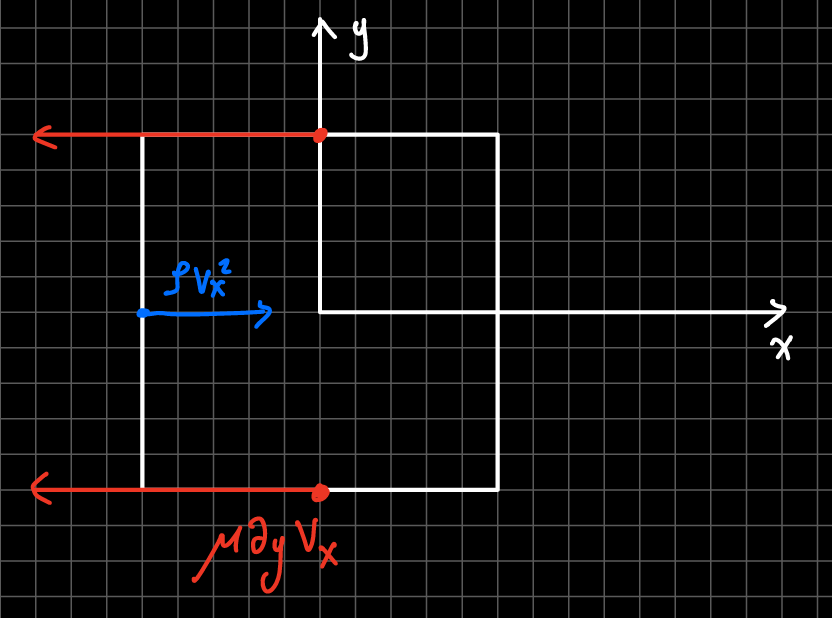
\includegraphics[width=0.75\textwidth]{Screenshot 2026-06-17 193220.png}
\end{figure}
\subsection{Heat}
The internal energy is 
\begin{equation}
	\del{t}\ins{\rho E}+\del{x_k}\ins{v_k\rho E - \kappa \del{x_k}T} = \sigma_{ik}\pdv{v_i}{x_k}
\end{equation}
Since we have Poiseuille flow  we can eliminate the elements depending on the derivative of the velocity since in both the case of \(x\) and \(y\) its zero
\begin{equation}
	\del{t}\ins{\rho E}-\kappa\ins{\del{x}^2+\del{y}^2}T = \sigma_{xy}\pdv{v_x}{y}
\end{equation}
assuming the energy is conserved and using the symmetry for the \(x\) axis
\begin{equation}
	-\kappa\del{y}^2T = \sigma_{ik}\pdv{v_x}{y}
\end{equation}
or 
\begin{equation}
	\kappa\del{y}^2T + \mu\ins{\pdv{v_x}{y}}^2=0
\end{equation}
The flow dissipates the energy but the energy is transported away, meaning at each place it remains constant over time.
\subsection{Steady State profile}
we can insert the velocity profile found earlier
\begin{equation}
	\kappa\del{y}^2T + \mu\ins{\frac{\Delta P}{2L\rho\nu}\ins{h-2y}}^2=0 \implies \del{y}^2T = -\frac{\mu}{\kappa}\ins{\frac{\Delta P}{2L\rho\nu}}^2\ins{h^2-4hy+4y^2}
\end{equation}
therefore
\begin{equation}
	T = -\frac{\mu}{\kappa}\ins{\frac{\Delta P}{2L\rho\nu}}^2\ins{\frac{2}{3}hy^3-\frac{1}{3}y^4-\frac{1}{2}h^2y^2+Ay}+B
\end{equation}
boundary conditions
\begin{equation}
	T(h/2)=T_0 \qquad \del{y}T(y=h/2)=0
\end{equation}
so 
\begin{equation}
	-\frac{\mu}{\kappa}\ins{\frac{\Delta P}{2L\rho\nu}}^2\ins{2h\ins{h/2}^2-\frac{4}{3}\ins{h/2}^3-h^2\ins{h/2}+A}=0 \implies A=\frac{h^3}{6}
\end{equation}
and
\begin{equation}
	-\frac{\mu}{\kappa}\ins{\frac{\Delta P}{2L\rho\nu}}^2\ins{\frac{2}{3}h\ins{h/2}^3-\frac{1}{3}\ins{h/2}^4-\frac{1}{2}h^2\ins{h/2}^2+\frac{h^3}{6}\ins{h/2}}+B=T_0
\end{equation}
gives
\begin{equation}
	B = T_0-\frac{\mu}{\kappa}\ins{\frac{\Delta P}{2L\rho\nu}}^2\ins{\frac{1}{48}h^2\ins{7h^2-6}}
\end{equation}
thus 
\begin{equation}
	T = -\frac{\mu}{\kappa}\ins{\frac{\Delta P}{2L\rho\nu}}^2\ins{\frac{2}{3}hy^3-\frac{1}{3}y^4-\frac{1}{2}h^2y^2+\frac{h^3}{6}y}+T_0-\frac{\mu}{\kappa}\ins{\frac{\Delta P}{2L\rho\nu}}^2\ins{\frac{1}{48}h^2\ins{7h^2-6}}
\end{equation}
\subsection{Estimate}
I'm very short on time so I just plugged the numbers without typing everything out
\begin{equation}
	\Delta T \approx \num{1,4e-2}\unit{\kelvin}
\end{equation}